\newpage
\section{Concept learning}
Il Concept Learning per esempio è la ricerca in spazi impotetici. Lo guardiamo perché è 
un'opportunità per dare uno sguardo ad un semplice apprendimento simbolico e come base per la sucessiva
introduzione di modelli flessibili.\\\\
Un altro caso sono gli spazi discreti (rappresentazione simbolica del bersaglio funzione), sono struttura dello
spazio delle ipotesi.\\\\
Il problema dell'apprendimento prevede di imparare come migliorare con l'esperienza in qualche compito. Migliorare oltre una task T,
tenendo conto di una misura di performance P e basandosi sull'esperienza E.

\begin{definition}
    Il concept learning si definisce come inferire una funzione booleana da esempi di tringing
    positivi e negativi.
    $$c: X \to \{t,f\} \:\:or\:\: \{+, -\} \:\:or\:\: \{yes, no\} \:\:or\:\: \{0,1\}$$
    con X che è lo spazio di instanze.
\end{definition}
\hspace{-15pt}Un esempio di concepts potrebberro essere "gatto" in animale o "sport-divertente" in giorni.
\begin{figure}[h!]
    \centering
    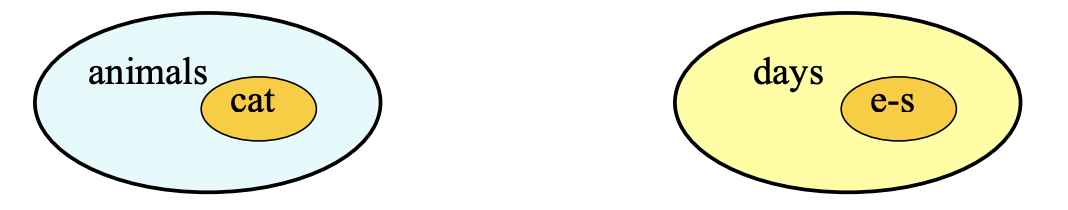
\includegraphics[width=0.5\textwidth]{images/ess-concept-learning.png}
\end{figure}
\begin{definition}
    Si definisce "\textbf{esempio}": $<x, c(x)>$ (o $<x,d>$) in D (o nell'insieme TR).
\end{definition}
\begin{definition}
    Si dice che $h: X\to \{0,1\}$ \textbf{soddisfa} $x$ se $h(x) = 1$
\end{definition}
\begin{definition}
    Una ipotesi $h$ è \textbf{consistente}
    \begin{itemize}
        \item Con un esempio $<x, c(x)>$, con $x \in X$ se $h(x) = c(x)$
        \item Con D, se $h(x) = c(x)$ per ogni esempio di training $<x, c(x)> \in D$
    \end{itemize}
\end{definition}
\begin{figure}[h!]
    \centering
    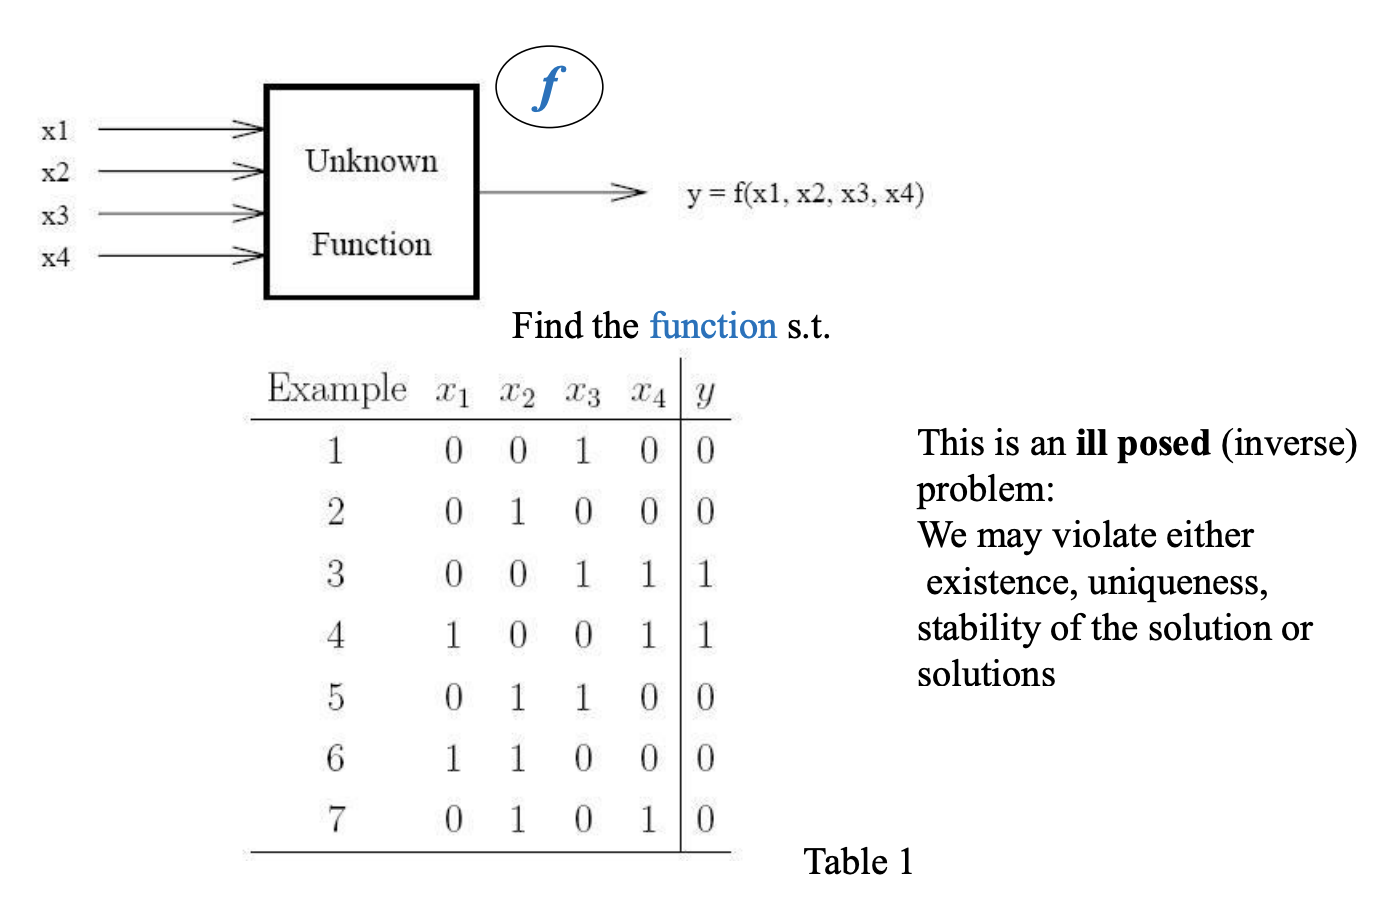
\includegraphics[width=0.65\textwidth]{images/learning-boolean-functions.png}
\end{figure}
\hspace{-15pt}Il problema dell'\textbf{ill posed} dice che: ci sono $2^{16} = 2^{2^4} = 65536$ possibili funzioni booleane
oltre quattro funzioni booleane di input. Noi non possiamo sapere quale sia corretta finché non abbiamo visto ogni possibile coppia
input-output. Dopo 7 esempi, noi continuiamo ad avere $2^9$ possibilità.
\begin{definition}
    Nel caso generale $|H| = 2^{\#-instances} = 2^{2^n}$ per inputs/outputs binari, e con n = dimensione input.
\end{definition}
\hspace{-15pt}\textbf{Per lavorare con spazi di ipotesi ristretti}: dobbiamo iniziare scegleindo uno spazio 
di ipotesi $H$ che è considerabile più piccolo rispetto allo spazio di tutte le possibili soluzioni.

\subsection{Regole congiuntive}
Quando ci chiediamo quante possibili $h$ abbiamo, è come chiedersi quante regole congiuntive semplici nell'esempio della tabella dei valori binari.\\
Nel caso generale:
\begin{itemize}
    \item Letterali positivi, per esempio: $h_1 = l_2 \:\:\: h_2 = (l_1 \land l_2) \:\:\: h_3 = true, \dots$\\
    \textbf{Regole congiuntive semplici} $|H| = 2^n$ (immaginando $l_i$ come un bit di una stringa di lunghezza n)
    \item Letterali (anche \textbf{not}($l_i$)) \hspace{15pt} $|H| = 3^n + 1$
\end{itemize}
\begin{example}
    Esempio di training per il concept.
    \begin{itemize}
        \item \textbf{Concept}: giorni il cui l'amico Aldo si diverte con il suo sport preferito.
        \item \textbf{Task}: prevedere il valore di "Enjoy Sport" per un giorno arbitrario in base ai valori degli altri attributi attributi.
    \end{itemize}
    \begin{figure}[h!]
        \centering
        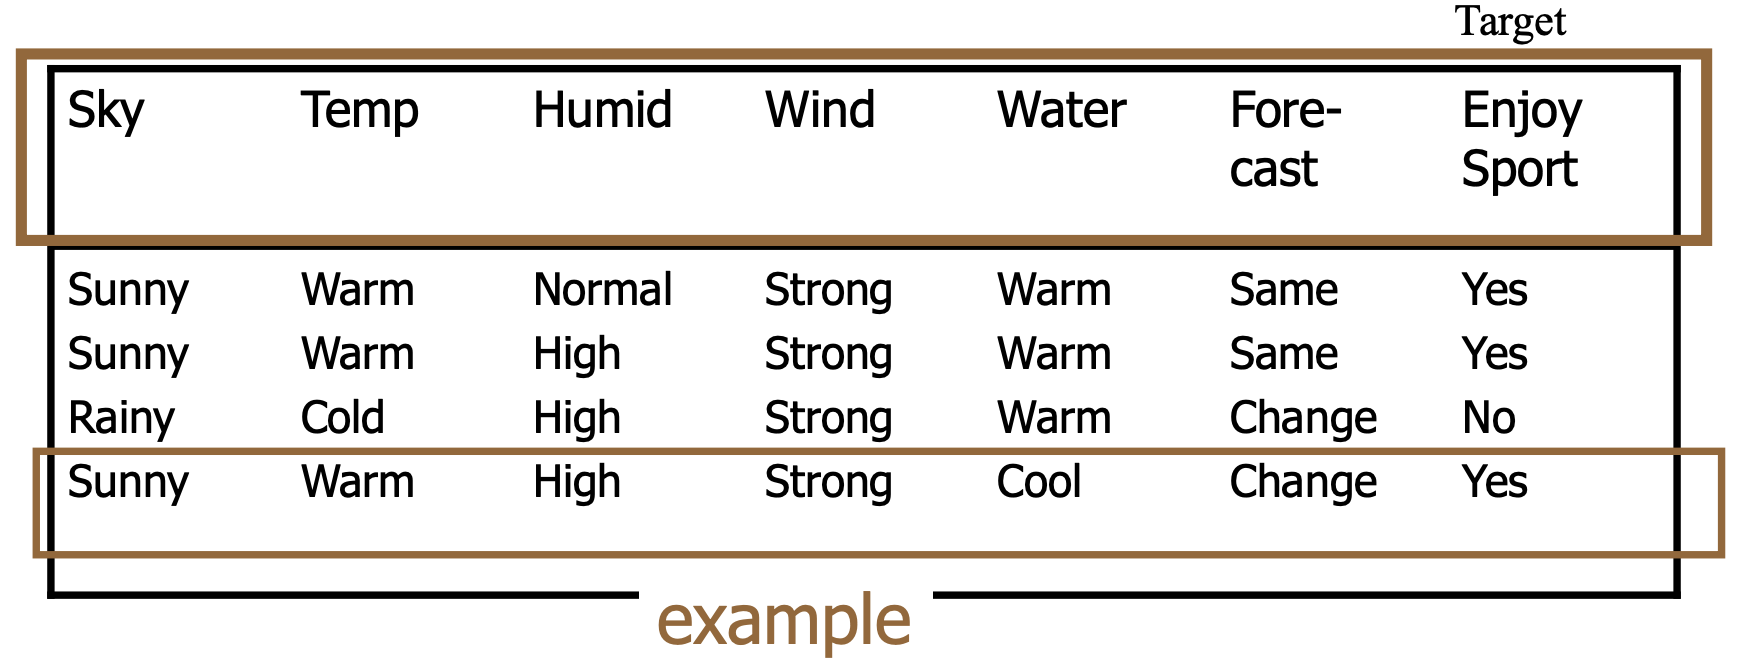
\includegraphics[width=0.5\textwidth]{images/training-esamples-concept-ler.png}
    \end{figure}
\end{example}
\subsubsection{Rappresentazione di ipotesi}
Un ipotesi $h$ è una congiunzione di vincoli sugli attributi. Ogni vincolo può contenere:
\begin{itemize}
    \item Uno specifico valore. Ess. Water=Warm
    \item Un valore che non mi interessa: Ess. Water=?
    \item Un valore non consetito (iporesi null). Ess. Water=$\O$
\end{itemize}
\begin{example}
    Un esempio di ipotesi $h$:\\
    Sky \hfill Temp \hfill Humid \hfill Wind \hfill Water \hfill Forecase\\
    Sunny \hfill ? \hfill ? \hfill Strong \hfill ? \hfill Same
    \begin{note}
        Questa è una funzione $h$, non un esempio di input.
    \end{note}
    \hspace{-15pt}Questa roba corrisponde alla funzione booleana:
    $$Sky = Sunny \land Wind = Strong \land Forecase = Same$$
    \begin{figure}[h!]
        \vspace{-15pt}
        \centering
        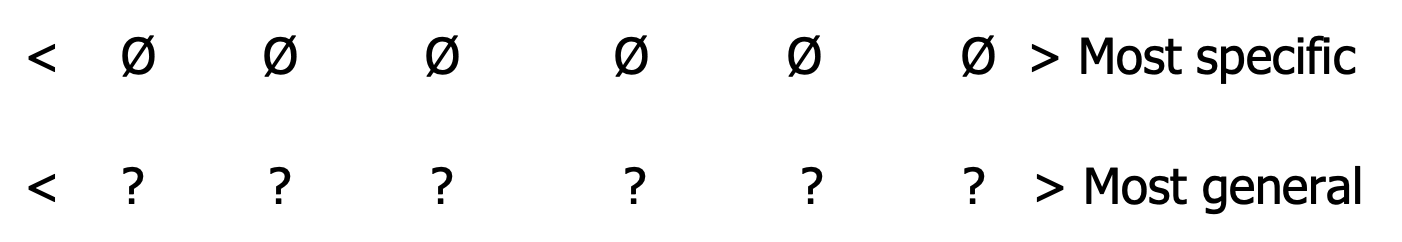
\includegraphics[width=0.5\textwidth]{images/rapre-ipotesi-ess.png}
    \end{figure}
\end{example}
\begin{definition}
    Task di apprendimento di concetti prototipici:
    \begin{itemize}
        \item \textbf{Given}
        \begin{itemize}
            \item \textbf{Istanza} X: Per esempio i possibili giorni descritti da degli attributi (Sky, Temp, Humidity, Wind, Water, Forecase)
            \item \textbf{Target function} c: EnjoySport X $\to \{0, 1\}$
            \item \textbf{Ipotesi H}: una congiunzione di (insieme finito di) letterali \\
            ess. $<$Sunny\:\: ? \:\:?\:\: Strong \:\:?\:\: Same $>$
            \item \textbf{Training examples} D: esempi positivi e negativi di una funzione target: $<x_1, c(x_1), \dots, <x_n, c(x_l)>$ ($l$ esempi)
        \end{itemize}
        \item \textbf{Trovare}: una ipotesi $h \in H$ tale che $h(x) = c(x)$ per ogni $x \in X$
    \end{itemize}
\end{definition}
Chiamiamo l'operazione di \textbf{Learning} la ricerca di ipotesi nello spazio $H$.\\\\
\textbf{Ipotesi dell'apprendimento induttivo}: Assumiamo in queste lezioni che "qualsiasi ipotesi trovata per approssimare la funzione target rispetto agli
esempi, andrà inoltre ad aprossimare la funzione target ben oltre gli esempi osservati".\\\\
$h=(x)$ per ogni $x \in D$ (ess. consistenza con D) \hspace{15pt} $h(x) = c(x)$ per ogni $x \in X$ \footnote{Un problema fondamentale del ML, analisi teorica ed empirica}\\\\
La rappresentazione per $H$ determina lo spazio di ricerca:
\begin{itemize}
    \item instance distinte: $3*2*2*2*2*2 = 96$
    \item Concetti distinti: $2^{96} = 2^{\#-instanze}$
    \item Ipotesi distinte sintatticamente (congiunzioni): $5*4*4*4*4*4 = 5120$ con 5 = sunny/cloudy/riny/?/$\O$ e 4=warm/cold/?/$\O$.
    \item Ipotesi distinte semanticamente: 1 + 4*3*3*3*3*3 = 973 (perché tutte le $h$ con $\O$ sono equivalenti a "false")
\end{itemize}
In generale: Dimensione elevata, addirittura infinita: strutturare lo spazio di ricerca può aiuto nella ricerca in modo più efficiente!

\subsubsection{Ordinamento da generale a specifico}
Consideriamo due ipotesi:
$$h_1 = <Sunny, ?, ?, Strong, ?, ?> \hspace{15pt} h_2 = <Sunny, ?, ?, ?, ?, ?>$$
Ed un insieme di instance coperte da $h_1$ e $h_2$.\\
$h_2$ impone meno vincoli rispetto a $h_1$ e quindi classifica più istanze x come positivo.
\begin{definition}
    Prendiamo $h_j$ e $h_k$ funzioni a valori booleani definite su X. Diciamo allora che $h_j$ è \textbf{più generale di o uguale a} $h_k$ (scritto come $h_j \geq h_k$) se e solo se
    $$\forall x \in X \: :\: [(h_k(x) = 1) \to (h_j(x) = 1)]$$
\end{definition}
\begin{example}
    Esempi binari $l_i: l_1 \geq (l_1 \land l_2),$ $l_1$ versus $l_2$, non comparabili. La relazione $\geq$ impone un 
    ordine di partizione (p.o.) sullo spazio di ipotesi $H$ che viene utilizzato da molti metodi di concept leargning. Possiamo approfittare di questo p.o. organizzare in modo efficiente la ricerca in H
\end{example}
\begin{figure}[h!]
    \centering
    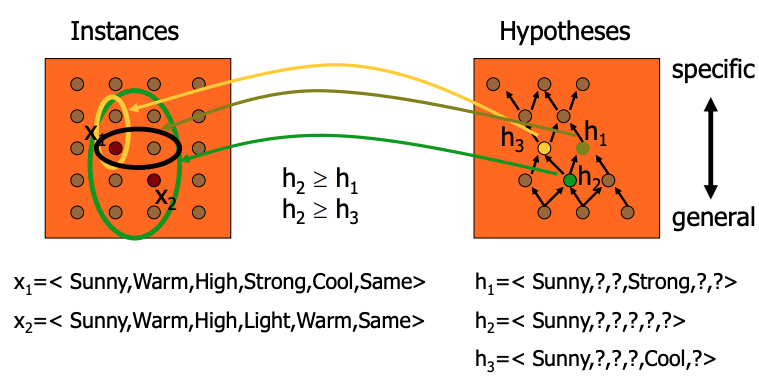
\includegraphics[width=0.6\textwidth]{images/struttura-su-H.png}
\end{figure}

\subsection{Algoritmo Find-S}
Sfrutta l'ordine parziale m.g.t per cercare in modo efficiente $h$ (senza fare un enumerazione esplicita per ogni $h \in H$).
\begin{definition}
    Definiamo l'Algoritmo con i seguenti passaggi:
    \begin{enumerate}
        \item Inizializzo $h$ con l'ipotesi più specifica in H.
        \item Per ogni instanza di training $x$ \textbf{positiva}
        \begin{lstlisting}
        for each attribute a_i in h
            if a_i in h e soddisfatto da x
                non fare nulla
            else
                sostituisci a_i in h dal successivo vincolo piu generale, cioe
                soddisfatto da x [es. rimuovi da h i letterali non soddisfacenti x]
        \end{lstlisting}
        \item In output ritorna un ipotesi $h$.
    \end{enumerate}
\end{definition}
Ricerca su spazio di ipotesi fatto dall'algoritmo Find-S:
\begin{figure}[h!]
    \centering
    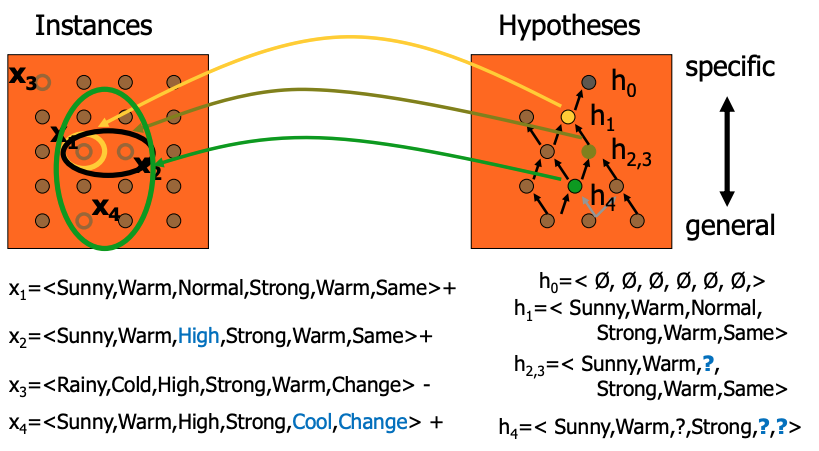
\includegraphics[width=0.65\textwidth]{images/ricerca-con-find-s.png}
\end{figure}

\hspace{-15pt}Alcune proprietà importnati dell'algoritmo find-S sono:
\begin{itemize}
    \item Lo spazio di ipotesi deve essere descritto da congiunzioni di attributi (forte limitazione)
    \item Find-S produttà l'iposeti più specifica fra quelle di H che sia anche coerente con gli esempi di training \textbf{positivi}.
    \item L'ipotesi di output $h$ sarà coerente con gli esempi negativi, a condizione che il terget conecpt sia contenuto in H. (perché $c \geq h$)
\end{itemize}
Mentre invece alcuni dei problemi relativi al Find-S sono i seguenti:
\begin{itemize}
    \item Non si può dire se l'apprendimento è convergente verso un concept target, nel senso
    che non è in grado di determinare se ha trovato l'unica ipotesi coerente con gli esempi di training.
    \item Non è possibile stabilire quando i dati di training sono incosistenti, poiché ignora gli esemi di training negativo: nessuna tolleranza al rumore!
\end{itemize}
Perché preferire l’ipotesi più specifica? Cosa succede se ci sono più ipotesi massimamente specifiche?

\subsection{Algoritmo List-Then eliminate}
Per parlare di questo algoritmo bisogna prima parlare del \textbf{version spaces}. L'idea chiave è che: l'output
è un descrizione dell'insieme di tutte le $h$ consistenti con D. Possiamo fare questo senza enumerare tutti loro:
$$Consistent(h, D) := \forall <x, c(x)> \in D\:\: h(x) = c(x)$$
\begin{definition}
    Il \textbf{version space}, $VS_{H,D}$ che rispetta lo spazio di ipotesi $H$, e l'insieme di training D, 
    è un sottoinsieme delle ipotesi di H consistenti con tutti gli esempi di traning:
    $$VS_{H,D} = \{h \in H \:\:|\:\: Consistent(h, D)\}$$
\end{definition}
\hspace{-15pt}L'algoritmo ora si definisce con i seguenti punti:
\begin{enumerate}
    \item Dato un VersionSpace $\to$ una lista contenente ogni ipotesi in H.
    \item Per ogni esempio di training $<x, c(x)>$ si rimiove dal VersionSpace ogni ipotesi
    che è inconsistente con l'esempio di training, $h(x) \neq c(x)$
    \item L'output è una lista di ipotesi in VersionSpace.
\end{enumerate}
Una miglior rappresentazione per il Version space (by G e S):
\begin{figure}[h!]
    \centering
    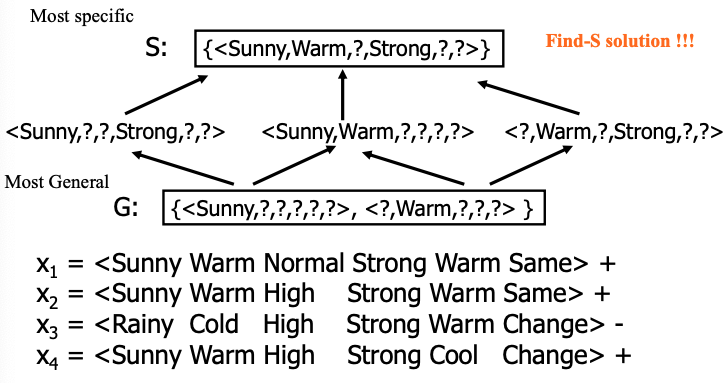
\includegraphics[width=0.65\textwidth]{images/miglior-rapresentazione-version-space.png}
\end{figure}

\subsection{Algoritmo candidate elimination}
\begin{definition}
    Ci sono vari modi per rappresentare il version space:
    \begin{itemize}
        \item Il \textbf{confine generale}, G, dello spazio delle versioni $VS_{H,D}$ è l'insieme di 
        membri generali massimi. (per H consistente con D).
        \item Il \textbf{confine specifico}, S, dello spazio delle versioni $VS_{H,D}$ è l'insieme di
        membri specifici massimi (per H consistente con D)
        \item \textbf{Teorema}: ogni membro della spazio di versione si trova fra questi confini.
    \end{itemize}
\end{definition}
$$VS_{H,D} = \{h \in H \:|\: (\exists \: s \in S) \:\: (\exists \: g \in G) \:\:(g \geq h \geq s)\}$$
dove $x \geq y$ vuol dire che $x$ è più o uguale generale rispetto a $y$
In questo algoritmo abbiamo che:
\begin{itemize}
    \item $G \to$ ipotesi massimali generali in $H$
    \item $S \to$ ipotesi massimali specifiche in $H$
\end{itemize}
For eatch esempio di training $d = <x, c(x)>$.
\begin{itemize}
    \item if d è un esempio \textbf{positivo} allora rimuovi da G qualsiasi ipotesi che sia incoerente con d (def di VS).\\
    for each ipotesi $s \in S$ che non è consistente con d [\textbf{generalizzare S}]
    \begin{itemize}
        \item Rimuovere s da S.
        \item Aggiungere ad S tutti le generalizzazioni minime h di s tale che: h consistente con d ed un qualche membri di G è più generale rispetto ad h.
        \item Rimuovere da S ogni ipotesi che è più generale rispetto ad altre ipotesi in S.
    \end{itemize}
    \item if d è un esempio \textbf{negtivo} allora rimuovere da S ogni ipotesi che è inconsistente con d.\\
    for eatch ipotesi $g \in G$ che non è consistente con d [specilizzazione G]
    \begin{itemize}
        \item rimuovere g da G.
        \item Aggiungere a G tutte le specializzazioni minime h di g tali che: h sia consistente con d e cia sia qualche membro di S che è più specifico rispetto a h.
        \item Rimuovere da G ogni ipoesi che è meno generale rispetto ad altre ipotesi in G.
    \end{itemize}
\end{itemize}
\begin{example}
    Esempio dell'algoritmo Candidate Elimination.
    \begin{figure}[h!]
        \begin{subfigure}{0.45\textwidth}
            \centering
            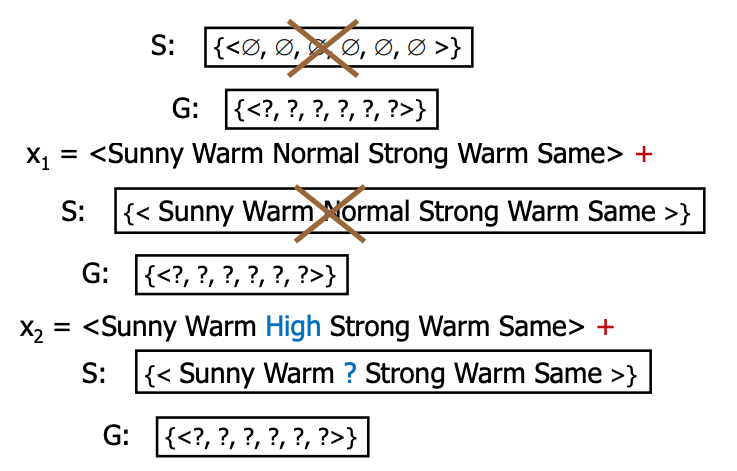
\includegraphics[width=\textwidth]{images/es-candidate-elimination-1.png}
        \end{subfigure}
        \hspace{10pt}
        \begin{subfigure}{0.45\textwidth}
            \centering
            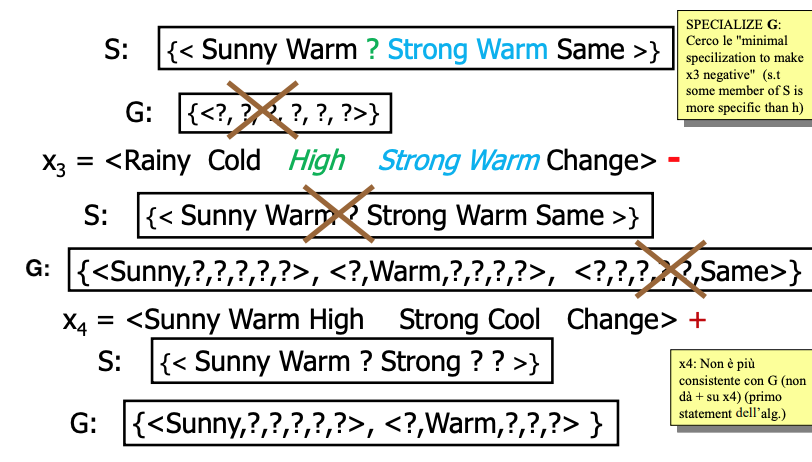
\includegraphics[width=\textwidth]{images/es-candidate-elimination-2.png}
        \end{subfigure}
    \end{figure}
\end{example}
La classificazione di nuovi dati si può fare nel seguente modo.
\begin{figure}[h!]
    \centering
    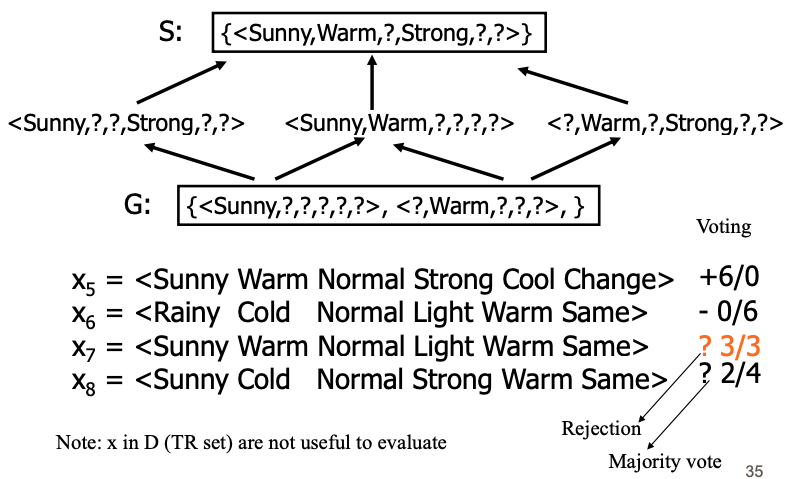
\includegraphics[width=0.6\textwidth]{images/classification-new-data.png}
\end{figure}

\subsection{Bias induttivo ed il suo ruolo}
Il nostro spazio di ipotesi non è capace di rappresentare un semplice concetto target di 
disgiunzione come il seguenti: $(Sky=Sunny) \lor (Sky=Cloudy)$. La candidate elimination sarebbe:
$$x_1 = <Sunny, Warm, Normal, Strong, <Cool, Change> + $$
$$x_2 = <Cloudy, Warm, Normal, Storng, Cool, Change> +$$
$S: \{<?, Warm, Normal, Strong, Cool, Change> \}$
$$x_3 = <Rainy, Warm, Normal, Strong, Cool, Change> -$$
$S: \{\}$\\\\
\textbf{Bias}: Assumiamo che lo spazio di ipotesi H contenga il concetto target c. In altre parole
che c sia descritto da con congiuzione (operatore AND) o da un letterale.

\subsubsection{Unbiased learning}
L'idea dietro al unbiased learning è la seguente: scegliere H che esprime ogni concetto che può
essere insegnato, ciò significa che H è l'insieme di tutti i possibili sottoinsiemi di X: il power set P(X).
\begin{example}
    $|H| = 96, |P(X)| = 2^{96} \sim 10^{28}$ concetti distinti.
\end{example}
\hspace{-15pt}H = disgiunzione, congiunzione, negazione. Ess. $<Sunny, Warm, Normal, ?, ?, ?> \lor <?, ?, ?, ?, ?, Change>$.
H contiene sicuramente il concetto target. A questo punto capiamo come generalizzare.\\\\
Che cosa sono S e G in questo caso?\\
Assumiamo esempi positivi $(x_1, x_2, x_3)$ ed esempi negativi $(x_4, x_5)$
$$S: \{(x_1 \lor x_2 \lor x_3)\} \hspace{15pt} G: \{\lnot (x_4 \lor x_5)\}$$
Gli unici esempi che sono classificati in modo non ambiguo sono gli esempi di training stessi (H può rappresentrli). In altre parole
per apprengere il concetto target si dovrebbe presentare ogni singola instanza in X come esempio di training.
\begin{definition}
    Un proprietà importante è che un \textbf{unbiased learner non è in grado di generalizzare}.
\end{definition}
\begin{demostration}
    Ogni instanza non osservata verrà classificata positiva per precisamente metà delle ipotesi nel VS e negativa nell'altrà metà (rejecion).
    Infatti: $\forall h$ consistenti con $x_i$ (test), $\exists h'$ identico ad h eccetto per il fatto che $h'(x_i) <> h(x_i)$, $h\in VS \Rightarrow h' \in VS$ (ci sono identici in D, l'insieme TR).
\end{demostration}
\hspace{-15pt}Un entità che apprendet e che non fa ipotesi preliminari riguardo all'identità del concetto target non ha basi
razionali per classificare ogni instanza invisibile. (Restrizione, preferenza) Bias non vengono solo assunti per l'efficienza, 
essi servono anche per la generalizzazione, tuttovia, non ci dice ancora (quantifica) quale sia la soluzione migliore generalizzanta.
\begin{example}
    \textbf{Esempio trivial} (TR = Training set, TS = Test set)
    \begin{figure}[h!]
        \centering
        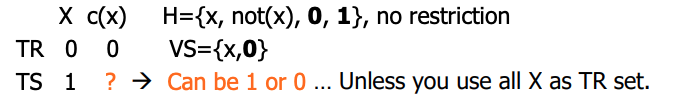
\includegraphics[width=0.5\textwidth]{images/trivial-esempio.png}
    \end{figure}
\end{example}
\hspace{-15pt}Problema: caratterizzare i bias per i diversi approcci di apprendimento.
\subsubsection{Bias induttivo}
Consideriamo le seguenti cose:
\begin{itemize}
    \item Un algoritmo di concept leargning L.
    \item Instance X, concetto target c.
    \item Esempi di trining $D_c = \{<x, c(x)>\}$
    \item Sia $L(x_i, D_c)$ a denotare l'assegnamento di classificazione all'instanza $x_i$ da L dopo il training con $D_c$.
\end{itemize}
\begin{definition}
    Il bias intduttivo di L è ogni insieme minimo di affermazioni \textbf{B} tali che per ogni concetto target c e corrispettivi dati di training $D_c$
    $$(\forall x_i \in X)[B \land D_c \land x_i] \vdash L(x_i, D_c)$$
    Dove $A \vdash B$ vuol dire che A implica logicamente B (segue deduttivamente da)
\end{definition}
\newpage
Sistema induttivo e \textbf{equivalente} sistema deduttivo.
\begin{figure}[h!]
    \centering
    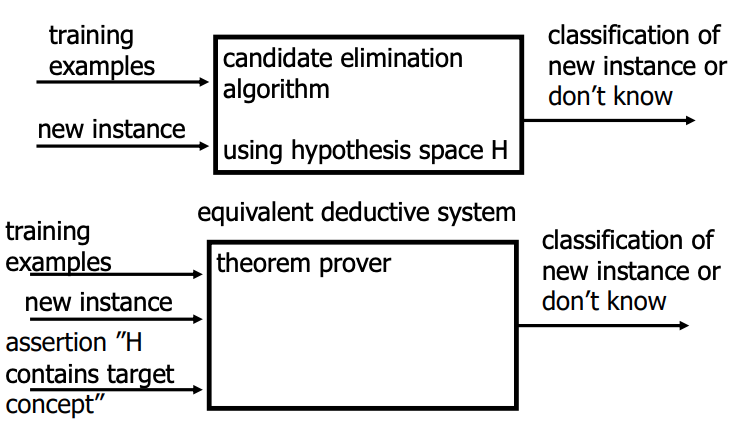
\includegraphics[width=0.65\textwidth]{images/inductive-system.png}
\end{figure}
Visto questo, vediamo 3 apprendimento con il bias diversi:
\begin{itemize}
    \item \textbf{Rote learner} (lookup table): memorizzare esempi, classificare x se e solo se esso matcha con un precedente esempio osservabile. No bias induttivo $\to$ no generalizzazione.
    \item \textbf{Version space candidate elimination algorithm}. Bias: lo spazio di ipotesi contiene il concetto target $|H| = 973$ versus $10^{28}$
    \item \textbf{Find-S}: Bias: Lo spazio delle ipotesi contiene il concetto target e tutto il resto delle istanze sono istanze negative a meno che non sia implicato il contrario
    dalle sue altre conoscenze (viste come esempi positivi). In altre parole: abbiamo una bias linguistico dovuto all'AND sul
    letterali più il bias di ricerca dovuto alla preferenza della ipotesi più specifica.
\end{itemize}